\section{Resultados}

%%%%%%%%%%%%%%%%%%%%%%%%%%%%%%%%%%%%%%% Formato Canônico
\begin{frame}{Modelo do Sistema em Malha Aberta - Formato Canônico}

$  \frac{C(s)}{R(s)}=\frac{K}{s+a}=\frac{0,4}{s+0,4} $
\hspace{1cm}
$\frac{C(s)}{R(s)} = \frac{1}{\tau s+1} = \frac{1}{2,5 s+1} = g(t)$

\vspace{-0.5cm}
\begin{figure}[!htb]
%\caption{Ação de Controle em Malha Aberta}
\center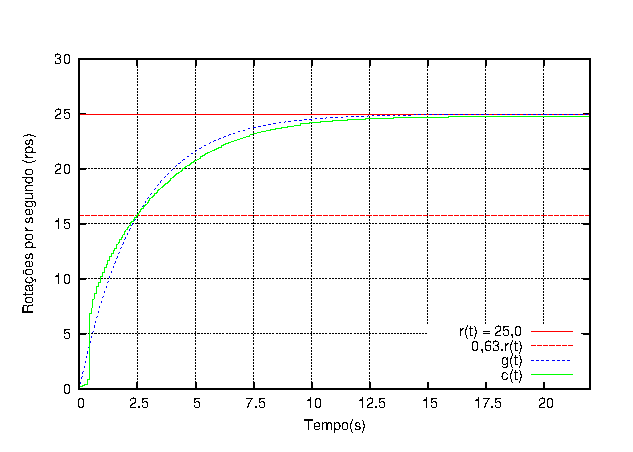
\includegraphics[scale=0.9]{./imagens/acaoMalhaAbertaTau.eps}
\label{fig:acaoMalhaAberTau}

%{\small Fonte: Próprio autor}
\end{figure}


\end{frame}




%%%%%%%%%%%%%%%%%%%%%%%%%%%%%%%%%%%%%%% Qualidade do Modelo
\begin{frame}{Qualidade do Modelo}
Erro Relativo Percentual

\begin{equation}
 \% erro = \frac{100}{N} . \sum_{n = 0,00}^{n=22,40} {\frac{| \text{\emph{r[n]}} -\text{\emph{c[n]}} |}{\text{\emph{r[n]}}} } 
\end{equation}

Onde:

\setlength{\parindent}{2cm}
r : valor real; 

c : valor calculado;

n : número da amostra aquisitada;

N : número total de amostras.


\end{frame}



%%%%%%%%%%%%%%%%%%%%%%%%%%%%%%%%%%%%%%% Qualidade do Modelo
\begin{frame}{Qualidade do Modelo}

\begin{table}[h]
\centering
\caption{Erro Relativo Percentual para intervalos determinados por $\tau$ }
\label{tab:ErroModeloTau}

\begin{tabular}{c|c}
\hline
Intervalo de amostras  &  erro médio relativo \\ \hline
\hline
%0 a 1 $\tau$ & 83,40 \% \\ \hline
1 a 2 $\tau$ &  3,16 \% \\ \hline
2 a 3 $\tau$ &  3,38 \% \\ \hline
3 a 4 $\tau$ &  2,00 \% \\ \hline
4 a 5 $\tau$ &  2,29 \% \\ \hline
$>$ 5 $\tau$ &  0,82 \% \\ \hline
\end{tabular}

%{\vspace{0.2cm} \small Fonte: Próprio autor}
\end{table}


\end{frame}










%%%%%%%%%%%%%%%%%%%%%%%%%%%%%%%%%%%%%%% Estabelecer uma meta
\begin{frame}{Requisitos de desempenho do sistema}% \tiny \cite{dorf2011modern}}
\vspace{-0.3cm}
\begin{itemize}
\item Tempo de subida: $\leqslant 2\tau$ do tempo de subida em malha aberta;
\item Sobressinal: $\leqslant$ 10\%;
\item Erro de regime estacionário: $\leqslant$ 5\%.
\end{itemize}

\vspace{-0.2cm}

\begin{figure}[!htb]
\centering
%\caption{Gráfico da função Resposta}
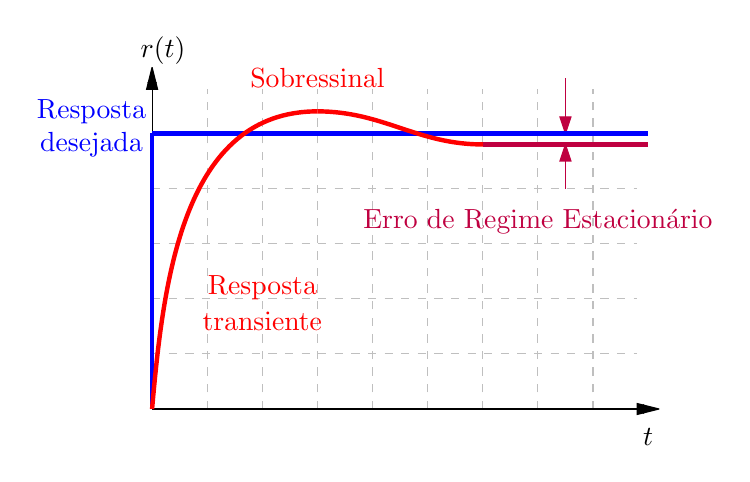
\begin{tikzpicture}[scale=0.70]
\draw [lightgray, dashed](0,0) grid (8.8,5.8);

\draw [->] (0,0) -- (9,0); 
\draw [fill] (0,6.2) -- (-0.1, 5.8) -- (0.1,5.8) -- (0,6.2);

\draw [->] (0,0) -- (0,6);
\draw [fill] (9.2,0) -- (8.8,0.1) -- (8.8,-0.1)--(9.2,0.0);

\draw [purple, ->] (7.5,4.0) -- (7.5,4.6); 
\draw [purple, fill] (7.5,4.8) -- (7.4,4.5) -- (7.6,4.5)--(7.5,4.8);

\draw [purple, ->] (7.5,6.0) -- (7.5,5.2); 
\draw [purple, fill] (7.5,5.0) -- (7.4,5.3) -- (7.6,5.3)--(7.5,5.0);

\node at (9.0,-0.5) {$t$};
\node at (0.2,6.5) {$r(t)$};

\draw [blue, ultra thick] (0.0,5.0) -- (9.0,5.0);
\draw [blue, ultra thick] (0.0,0.0) -- (0.0,5.0);

\draw [red, ultra thick] (0.0,0.0) to [out= 85, in=180] (3,5.4);
\draw [red, ultra thick] (3.0,5.4) to [out=  0, in=180] (6,4.8);

\draw [purple, ultra thick] (6,4.8) -- (9,4.8);

\node at (-1.1,5.4)[blue]{{Resposta}};
\node at (-1.1,4.8)[blue]{{desejada}};
\node at (2.0,2.2)[red]{{Resposta}};
\node at (2.0,1.6)[red]{{transiente}};
\node at (3.0,6.0)[red]{{Sobressinal}};
\node at (7.0,3.4)[purple]{{Erro de Regime Estacionário}};

\end{tikzpicture} 
\label{fig:funcaoResposta}

%{\small Fonte: \cite{dorf2011modern} }
\end{figure}



\end{frame}






%%%%%%%%%%%%%%%%%%%%%%%%%%%%%%%%%%%%%%% Controlador PI e LPAEt
\begin{frame}{Controlador PI e LPA$E\tau$}

\vspace{-0.5cm}
\begin{figure}[!htb]
%\caption{Ação de Controle em Malha Aberta}
\center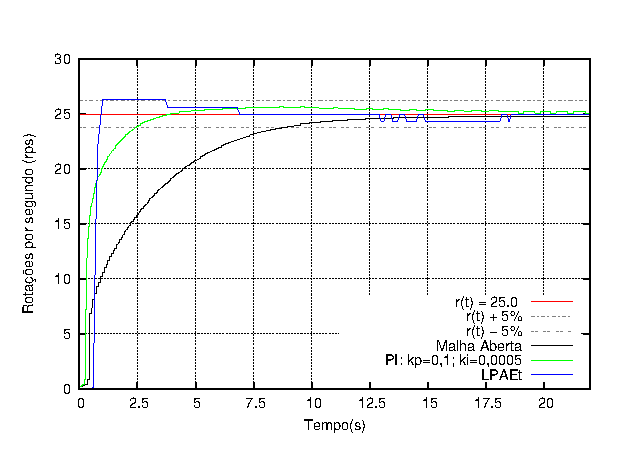
\includegraphics[scale=1.0]{./imagens/resAcaoPI.eps}
\label{fig:resAcaoPI}

%{\small Fonte: Próprio autor}
\end{figure}


\end{frame}


%%%%%%%%%%%%%%%%%%%%%%%%%%%%%%%%%%%%%%% Controlador LPAEt repetitivo
\begin{frame}{Controlador LPA$E\tau$}

\vspace{-0.5cm}
\begin{figure}[!htb]
%\caption{Ação de Controle em Malha Aberta}
\center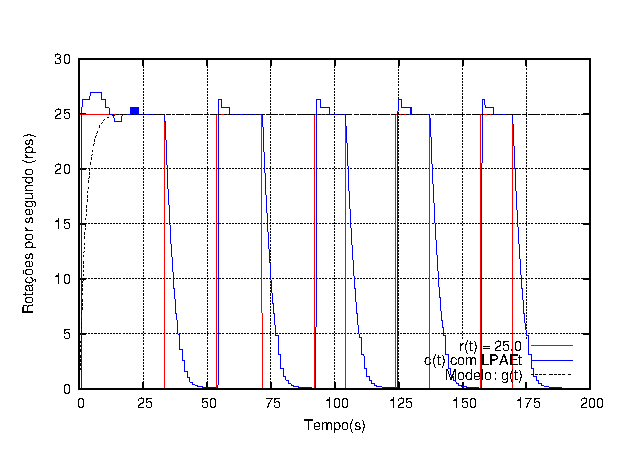
\includegraphics[scale=1.0]{./imagens/LPAEt-delta.eps}
\label{fig:lpaetDelta}

%{\small Fonte: Próprio autor}
\end{figure}


\end{frame}



%%%%%%%%%%%%%%%%%%%%%%%%%%%%%%%%%%%%%%% Controlador LPAEt Erro
\begin{frame}{Controlador LPA$E\tau$}

\vspace{-0.5cm}
\begin{figure}[!htb]
%\caption{Ação de Controle em Malha Aberta}
\center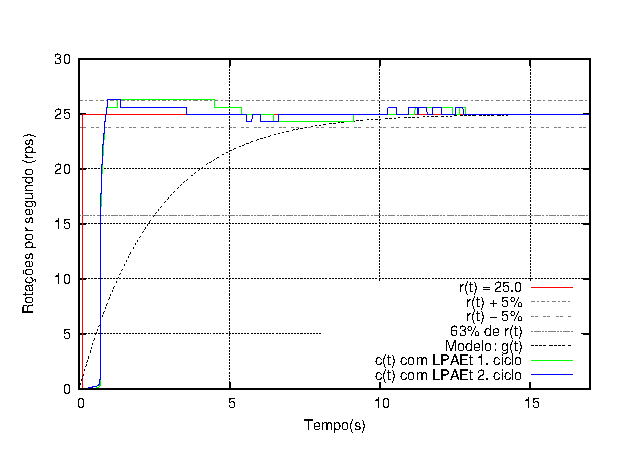
\includegraphics[scale=1.0]{./imagens/LPAEt-erro.eps}
\label{fig:lpaetErro}

%{\small Fonte: Próprio autor}
\end{figure}


\end{frame}
